% Chapter 3

\chapter{Methods used to measure the MOS structure.}% Main chapter title
\label{Chapter3}% For referencing the chapter elsewhere, use \ref{Chapter1}
\lhead{Chapter 3. \emph{Methods used to measure MOS structure}}% This is for the header on each page - perhaps a shortened title

%----------------------------------------------------------------------------------------

Capacitance-voltage (C-V) methods, which will be used in this thesis
deal with, provide comprehensive information on the electrophysical
parameters of the MOS structure.  To determine some of the parameters
the evaluation of data measured by one method is sufficient, but in
most cases, a combination of several methods can be used to obtain
more accurate results.  In the previous chapter, we used the example
of C-V dependence of the ideal MOS structure, we demonstrated the
differences between voltage dependences of the capacitance of the MOS
structure measured by different methods:

\begin{itemize}
\item low-frequency (possibly quasi-static) C-V method
\item equilibrium high-frequency C-V method
\item non-equilibrium high-frequency C-V method.
\end{itemize}

In addition to the above methods, we used the Q-C method in this
dissertation, which combines the properties of high-frequency and
low-frequency C-V method. Determination of the same C-V dependencies
using different methods at the same time represents a kind of control
of the measurement accuracy.  This is advantageous especially in cases
where the determination of the absolute measurement error represents a
complex problem. For the measurement of the generation lifetime of
minority charge carriers, we used the constant width OPN
method~\cite{3.1}, which has the advantage over the classical Zerbst
C-t method~\cite{3.2} is the faster measurement speed. A modification
of the constant width method OPN~\cite{3.3} width modification also
eliminates the effect of lateral injection of minority charge carriers
into the OPN from the substrate.

The advantage of the above methods is that they are not destructive,
which in conjunction with their speed, makes them suitable for routine
use in industry.  V laboratory conditions, it is appropriate to
validate these methods using other methods which may be considered
complementary. This is the case for measurement of the concentration
profile of impurities, for example by the scattering method
resistivity method, the electrochemical capacitance method or
SIMS\@. It is appropriate Also, verification of the concentration
profile by simulation of the process of the process. When
investigating the energy states present in the forbidden band of the
semiconductor, good information is provided by the DLTS method.

The above C-V methods represent a subset of the broad field of
diagnostics of MOS structures using capacitance measurements. The
following schematic illustrates their relationship to the parameters
under investigation, which have been the subject of of this work and
also highlights the areas of concern that were needed to be addressed.

\begin{diagram}
  \centering
  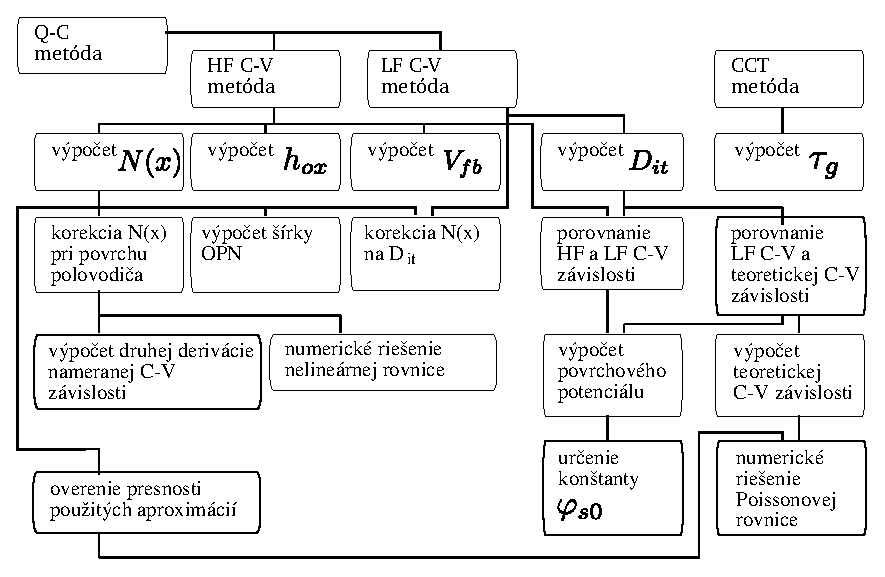
\includegraphics[width=\textwidth,height=\textheight,scale=0.7,keepaspectratio]{Figures/diagram-1.EPS}\label{diagram:1}
\end{diagram}

\section{High frequency C-V method.}\label{sec:3.1}

In the high-frequency capacitive method measurement, the MOS structure
is brought to the desired state by a DC gate voltage and its
capacitance is determined from the current response to a
high-frequency signal of small amplitude, which is superimposed on the
DC gate voltage. By measuring the phase shift between the
high-frequency voltage signal and current, in addition to the
capacitance, it is also possible to evaluate the conductivity of the
structure. The magnitude of the frequency of the measurement signal is
determined by the trade-off between the requirement of the highest
possible frequency from the influence measurement by the fast traps of
the $Si-SiO_2$ interface and the technical possibilities of standard
measuring instruments.  In our experiment we used the HP4280a
instrument, whose measurement signal has a fixed frequency 1 MHz and
the amplitude of the measurement signal can be selected as 10 mV, or
30 mV.  The above mentioned instrument can be controlled using the
IMS-2 bus. It should be It should be noted that the instrument, in
conjunction with the PC AT control system, is capable of block
transfer to measure and transfer in binary format to the control 680
points (which is the limit for block transfer) of C-V and G-V
dependencies in 25 seconds.  The above time figure is based on our own
experiments.

\section{Quasi-static C-V method.}\label{sec:3.2}

In the quasi-static capacitance method measurement, the MOS structure
is charged by a slow, increasing gate voltage over time. The
capacitance of the MOS structure is determined as a function of the
charging current and the rate of rise of the gate voltage.  Hence, to
implement the method, it is a source of continuously increasing
voltage is required and ammeter. The rate of voltage rise must be
small enough to the structure is still in thermodynamic equilibrium
during the measurement. At On the other hand, as the rate decreases,
the current which we have to measure. For most of the samples
measured, a velocity of the order of $10^{-2}V/s$, which for a
capacitance of $100pF$ represents the charging current $10^{-12}A$. In
our experiment, we used a charge-current Keithley 642 electrometer,
which measures current in the range of $10^{-8}A$ to $10^{-17}A$ with
a resolution of 5 digits per range.  It should be noted that in
addition to the other excellent features of the instrument, the
manufacturer guarantees an effective noise figure of less than
$8\times10^{-17}A$. The source of the increasing voltage, which was
built in our department, allows the adjustment of the rate of voltage
rise in the range from $10V/s$ to $10^{-3}V/s$ with with a resolution
of 1\% of the range. Both devices can be controlled using the bus
IMS-2.  The main source of error in the quasi-static method is the
inaccuracy of the determination of the gate voltage rise
rate~\cite{1.5}. Before each measurement, it is necessary to
accurately measure the rate of voltage rise, which is then used in the
capacitance calculation. The rate of voltage rise for selected range
is determined in our case from the ratio of the voltage change and the
time in 10 s. This value then has the meaning of a mean value and its
use in the calculation assumes a linear increase in voltage, which we
experimentally verified for a representative sample of voltage rise
ranges of voltage over time.

\section{Q-C method.}\label{sec:3.3}

Q-C method\cite{3.4} is a combination of high frequency C-V method and
the charge Q-V method~\cite{3.5}. Its principle is is as follows. In
series with a condenser formed by a MOS structure, the
voltage-independent capacitance, which we denote by $C_i$.  At
series-parallel connection of the capacitors, which is shown in
Figure~\ref{fig:3.1}, we connect a DC voltage $V_a$ and measure the
voltage $V_i$ at the common point of the capacitor connections, which
represent capacitive divider. The capacitors labeled $C_w$ and $C_x$
show parasitic capacitances. $C_w$ is the capacitance between the
table and the raised probe tip and $C_x$ is the capacitance of the
common point of connection of the capacitors with respect to
ground. At the same time as measuring the voltage $V_i$, we also
measure capacitance $C_m$ and conductivity $G_m$ using a high
frequency signal superimposed on the voltage $V_a$.

\begin{figure}[h!]\centering
  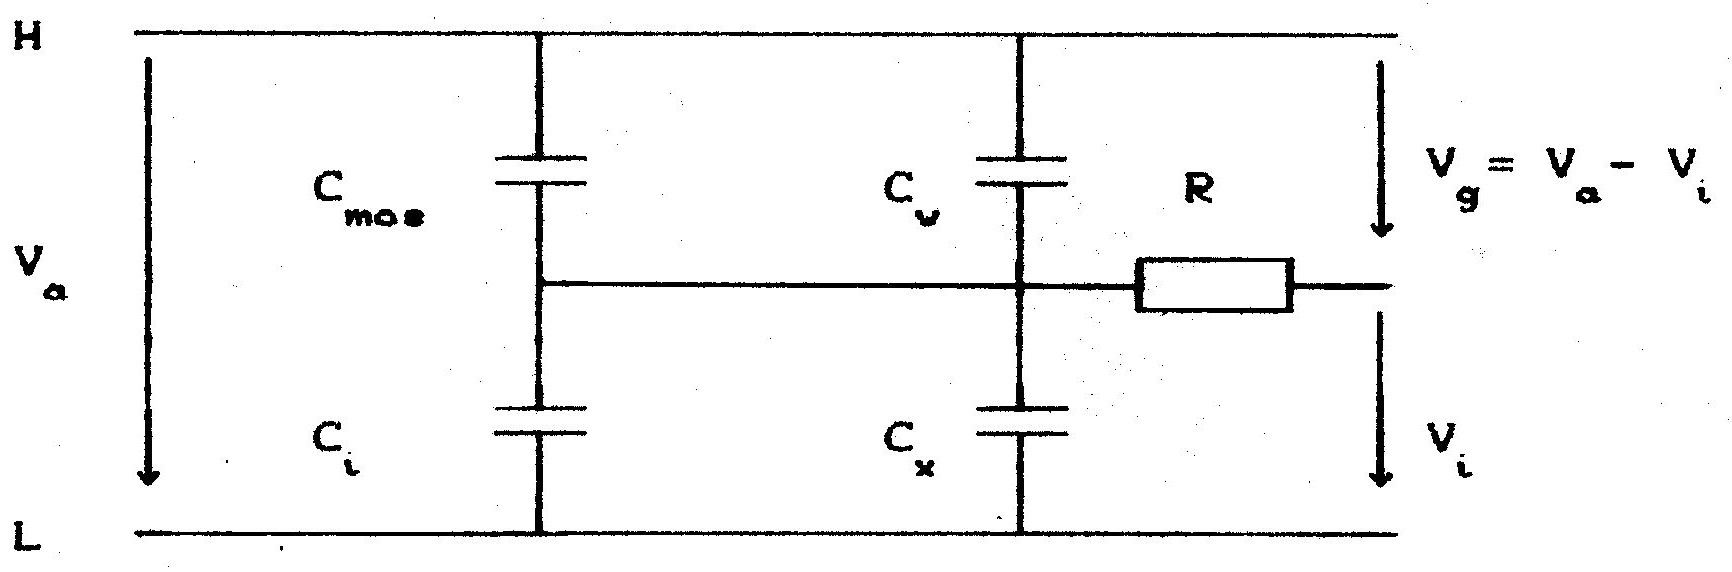
\includegraphics{Figures/fig-3-1.eps}% chktex-file 8
  \caption[Schematic illustration of Q-C capacitor wiring
    methods]{Schematic representation of Q-C capacitors wiring
    methods}\label{fig:3.1}
\end{figure}

Between the common point of the capacitor wiring and the voltmeter
input is a resistor is connected which, together with the capacitance
of the voltmeter lead wires and the input capacitance of the voltmeter
form a low-pass filter, causing the measured voltage to be unaffected
by high-frequency signal. It also follows that the magnitude of the
capacitance between the common point of connection and point L will be
different for DC and high-frequency measurements. Let us therefore
denote the capacitance $C_i$ for DC measurement $C_{iLF}$ and for high
frequency measurement $C_{iHF}$.  Mentioned resistance together with
the input resistance of the voltmeter forms the voltage divider.  To
the voltage measurement is not affected, a voltmeter with high input
resistance.  The suitability of using the Keithley 642 meter, whose
input resistance in the measurement mode is approximately $10^{16}
\Omega$ and its parasitic input capacitance is $2 pF$. A detailed
description of the circuit of the Q-C method, eliminating of parasitic
capacitances, or the methodology of their measurement, is described in
Appendix~\ref{app:AppendixE}. If we know the capacitance of the oxide
layer of the MOS structure $C_{ox}$ and the magnitude of the
capacitance $C_{iLF}$, we can calculate the value of the surface
potential $\varphi_s$ from the following relation, derived in
Appendix~\ref{app:AppendixF}.

\begin{equation}\label{eq:3.1}
  \varphi_s = \varphi_{s0} + V_g (1 + \frac{C_w}{C_{ox}}) - V_i \frac{C_{iLF}+C_x}{C_{ox}}
\end{equation}

At the same time, we can determine the low-frequency capacitance of
the MOS structure

\begin{equation}\label{eq:3.2}
  C^{LF}_{mos} = C_{ox} (1 - \frac{d\varphi_s}{dV_g})
\end{equation}

The defect charges present in the measured MOS structure cause the
surface potential of the semiconductor assumes the value
$\varphi_{s0}$ even at zero gate voltage. The magnitude of this
constant can be determined from a comparison of the measured and
theoretical dependence of the surface potential on the OPN width
$\varphi(x)$.  The method for determining $\varphi_{s0}$ is described
in Appendix~\ref{app:AppendixG}. It may be noted here that to
calculate $C^{LF}_{mos}$ the value of this constant is not needed, as
can be seen from relations~\ref{eq:3.1} and~\ref{eq:3.2}.

From the measured values of $C_m$ and $G_m$ we can determine the high
frequency capacitance of the MOS structure using the following
relations.  First calculate the corresponding resistance $R_m$ and
reactance $X_m$

\begin{subequations}\label{eq:3.3}
  \begin{align}
    R_m &= \frac{G_m}{G^2_m + {(\omega C_m)}^2}\label{eq:3.3a}\\[0.3cm]
    X_m &= \frac{\omega C_m}{G^2_m + {(\omega C_m)}^2}\label{eq:3.3b}\\[0.3cm]
    \intertext{,which we use in the relation}
    C^{HF}_{mos} &= - \cfrac{R^2_m + {(X_m + \frac{1}{\omega C_{iHF}} + \omega C_w D^2)}^2}{\omega D^2{(X_m + \frac{1}{\omega C_{iHF}} + \omega C_{w} D^2)}^2}\label{eq:3.3c}\\[0.3cm]
    \intertext{,where}
    D^2 &= R^2_m + {(X_m + \frac{1}{\omega C_{iHF}})}^2\label{eq:3.3d}
  \end{align}
\end{subequations}

A detailed description and derivation of the above relationships is
described in the Appendix E. The Q-C method provides a number of
advantages.  It allows simultaneous measurement of high and low
frequency C-V dependence, guaranteeing the same measurement conditions
for both dependences, and eliminates the possibility of their mutual
voltage drift, which can occur if the dependencies were sensed
sequentially.  At the same time, the measurement of the low-frequency
C-V dependence is static and does not depend on the dynamics of the
gate voltage.

To determine the concentration profile of impurities in the subsurface
of the semiconductor, it is advantageous to know the surface potential
waveform, which allows calculation unencumbered by the traps of the
$Si-SiO_2$ interface. Cited by advantages are offset by the difficulty
of the method for the instrumentation used.  A critical point in the
implementation of the method is the stripping of the common point of
the capacitors. The connected voltage $V_a$ must be decomposed into
capacitors according to their capacitances and not according to their
leakage resistances.  This requires the use of a good quality
capacitor $C_i$ and the arrangement of of the individual components of
the method so that the leakage current from a common point to ground
is as small as possible. This makes the use of the Q-C method excludes
MOS structures that have large leakage currents due to imperfections
in the oxide layer. For measurements in the thermodynamic state
equilibrium, as stated by the authors of the method~\cite{3.7}, it is
necessary to the voltage $V_i$ to remain unchanged for at least 10
seconds by an order of magnitude $10^{-3}V$. For the purpose of
determining the concentration profile, we can measure non-equilibrium
C-V dependence, where the leakage currents from the common point to
ground do not manifest themselves to such an extent because the
measured voltage is read immediately after the voltage is applied. In
Figure~\ref{fig:3.2} the shows the normalized waveforms of the HF C-V
dependence of the MOS structure and surface potential waveforms with
respect to the gate voltage determined by Q-C method for measurements
in the thermodynamic equilibrium state and in the deep depletion. The
instruments used in the implementation of the method on our
department~\cite{3.8,3.9} can be controlled using the IMS-2 bus and
the measured values of voltages $V_a$, $V_i$, capacitance $C_m$ and
conductivity $G_m$ can be stored in a disk file for further
processing.

\begin{figure}[h!]\centering
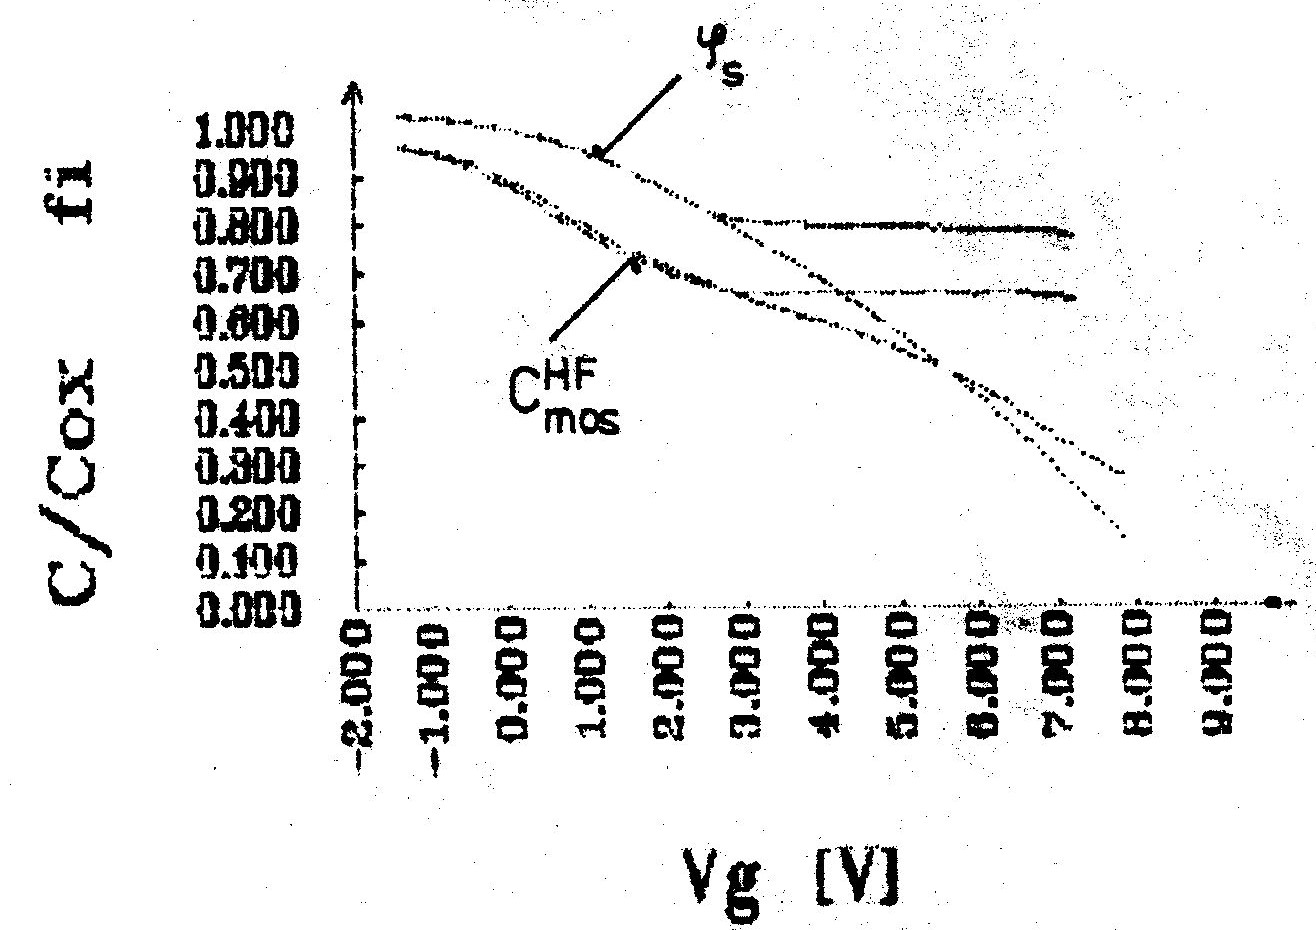
\includegraphics{Figures/fig-3-2.eps}
\caption[Normalized waveforms HF C-V dependence of MOS structure and waveform
  surface potential versus gate voltage determined using the Q-C method
  for measurements in thermodynamic equilibrium and deep
  depletion]{Normalized HF C-V waveforms of the structure
  MOS and surface potential waveforms from gate voltage determined
  using the Q-C method for measurements in the thermodynamic equilibrium state and in
  deep depletion state. The $\varphi_s(V_g)$ waveforms are shown
  using the normalization $1-\frac{\varphi_s}{\varphi_{norm}}$, where
  $\varphi_{norm}=3.33V$.}\label{fig:3.2}
\end{figure}
%OBR7.BIT

To verify the accuracy of the Q-C method, we have used the same MOS
structure we performed separate high and low frequency measurements
and simultaneously calculated the same capacitance dependencies from
the measured values Q-C method.  The resulting curves are shown in
Figures~\ref{fig:3.3} and~\ref{fig:3.4}.

For a quantitative comparison of the results shown in
Fig.~\ref{fig:3.3} and~\ref{fig:3.4}, we present in
Table~\ref{tab:3.1} and~\ref{tab:3.2} numerical values of the
normalized capacitances $C^{HF}_{mos}$ and $C^{LF}_{mos}$ for the HF,
LF and Q-C methods and their difference in terms of relative
error. The tables show the difference between the C-V dependencies,
which is due both to inaccuracies in the determination of of the
parasitic capacitances and secondly the leakage currents used
capacitors. The authors of the method recommend to eliminate leakage
of leakage currents caused by the humidity of the environment, use an
air capacitor $C_i$ and to direct a current to the sample to be
measured during the measurement to prevent condensation of water
vapour from the surroundings.

\newpage
\begin{figure}[h!]\centering
  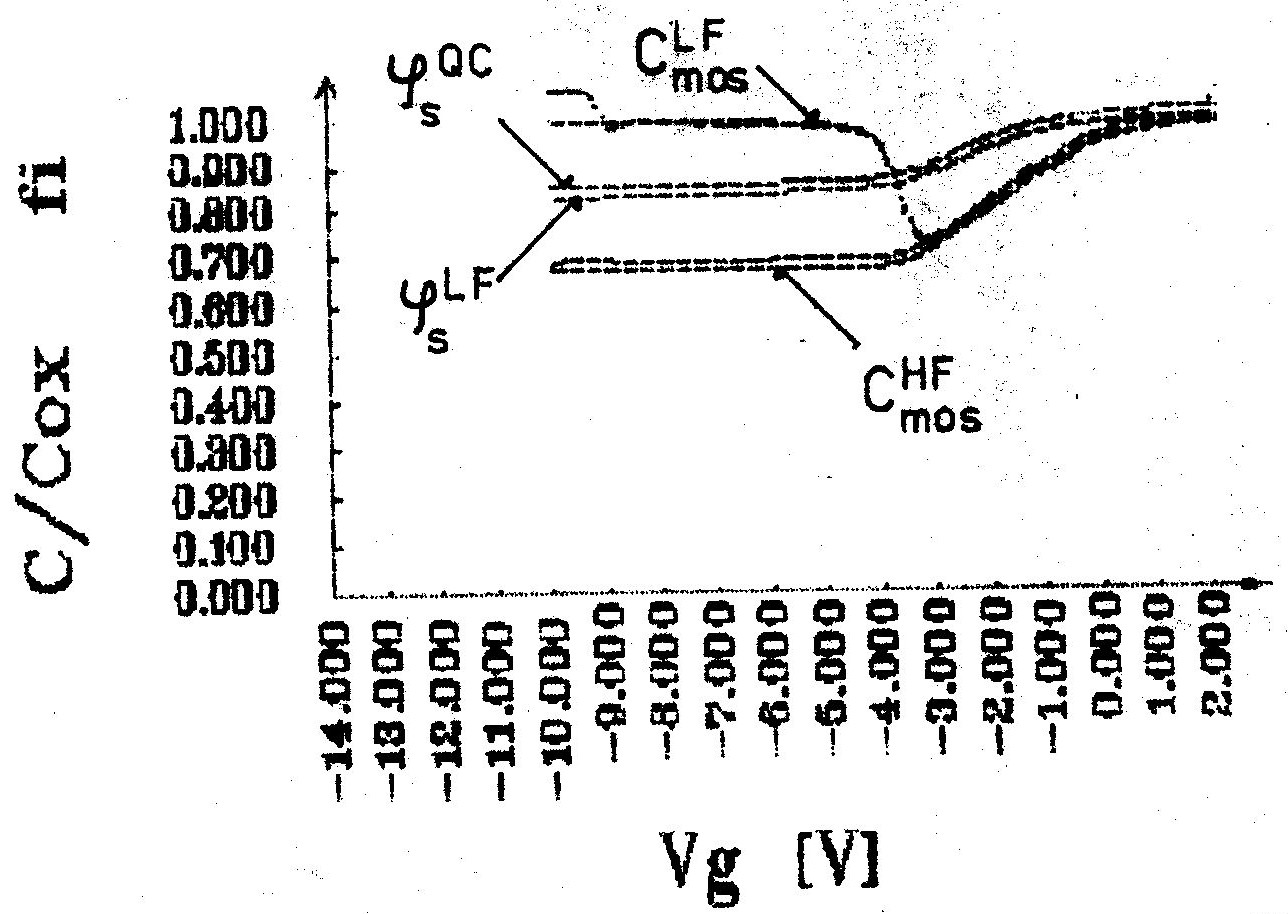
\includegraphics{Figures/fig-3-3.eps}
  \caption[Normalized capacitance waveforms of MOS structure with substrate type
  N as a function of gate voltage for equilibrium high-frequency and
  quasi-static measurements]{Normalized capacitance waveforms of a MOS structure with
  N-type substrate as a function of gate voltage for equilibrium
  high-frequency and quasi-static measurements.  At the same time, those
  same characteristics obtained by the Q-C method. For completeness, the
  the dependence of the surface potential
  ${\varphi_s(V_g)}^{QC}$ obtained using the Q-C method and the dependence
  ${\varphi_s(V_g)}^{LF}$ calculated by integrating the low-frequency C-V
  dependence using the Berglund integral.  Flows
  $\varphi_s(V_g)$ are shown using the normalization $1-\frac{\varphi_s}{\varphi_{norm}}$, kde $\varphi_{norm}=-3.33V$.}\label{fig:3.3}
\end{figure}
%OBR5.BIT

\begin{table}[h!]\centering
  \begin{tabular}{c c c c c c}
    \multicolumn{3}{l}{$C^{HF}_{mos}$} & \multicolumn{3}{l}{$C^{LF}_{mos}$} \\
    HF[\%] & QC[\%] & $\Delta_r$[\%] & LF[\%] & QC[\%] & $\Delta_r$[\%] \\
    \hline% chktex-file 44
    99.67 & 98.30 & +1.37 & 97.85 & 99.14 & -1.32 \\
    98.56 & 96.69 & +1.89 & 96.59 & 97.05 & -0.47 \\
    98.56 & 96.69 & +1.89 & 96.59 & 97.05 & -0.47 \\
    95.73 & 93.89 & +1.92 & 93.93 & 94.51 & -0.61 \\
    89.89 & 87.75 & +2.39 & 88.26 & 88.57 & -0.36 \\
    82.15 & 80.17 & +2.41 & 81.43 & 81.82 & -0.47 \\
    74.83 & 73.09 & +2.33 & 73.79 & 74.57 & -1.06 \\
    69.69 & 67.81 & +2.70 & 86.08 & 86.33 & -0.29 \\
    69.10 & 67.20 & +2.74 & 97.20 & 97.73 & -0.54 \\
    68.97 & 67.08 & +2.74 & 98.27 & 98.74 & -0.48 \\
    68.91 & 67.03 & +2.72 & 98.75 & 99.38 & -0.64 \\
    68.90 & 67.01 & +2.75 & 99.04 & 98.68 & -0.36 \\
    68.90 & 67.03 & +2.70 & 99.20 & 99.87 & -0.67 \\
  \end{tabular}
  \caption[Comparison of normalized frequency and low-frequency
    capacitance of the MOS structure (Figure~\ref{fig:3.3}) for HF, LF
    and Q-C methods]{Comparison of normalized high-frequency and
    low-frequency capacitance of the MOS structure
    (Figure~\ref{fig:3.3}) for HF, LF and Q-C methods. The difference
    of the curves is expressed by the relative error.}\label{tab:3.1}
\end{table}

\newpage
\begin{figure}[h!]\centering
%\framebox[10cm]{\rule{0cm}{3cm}}
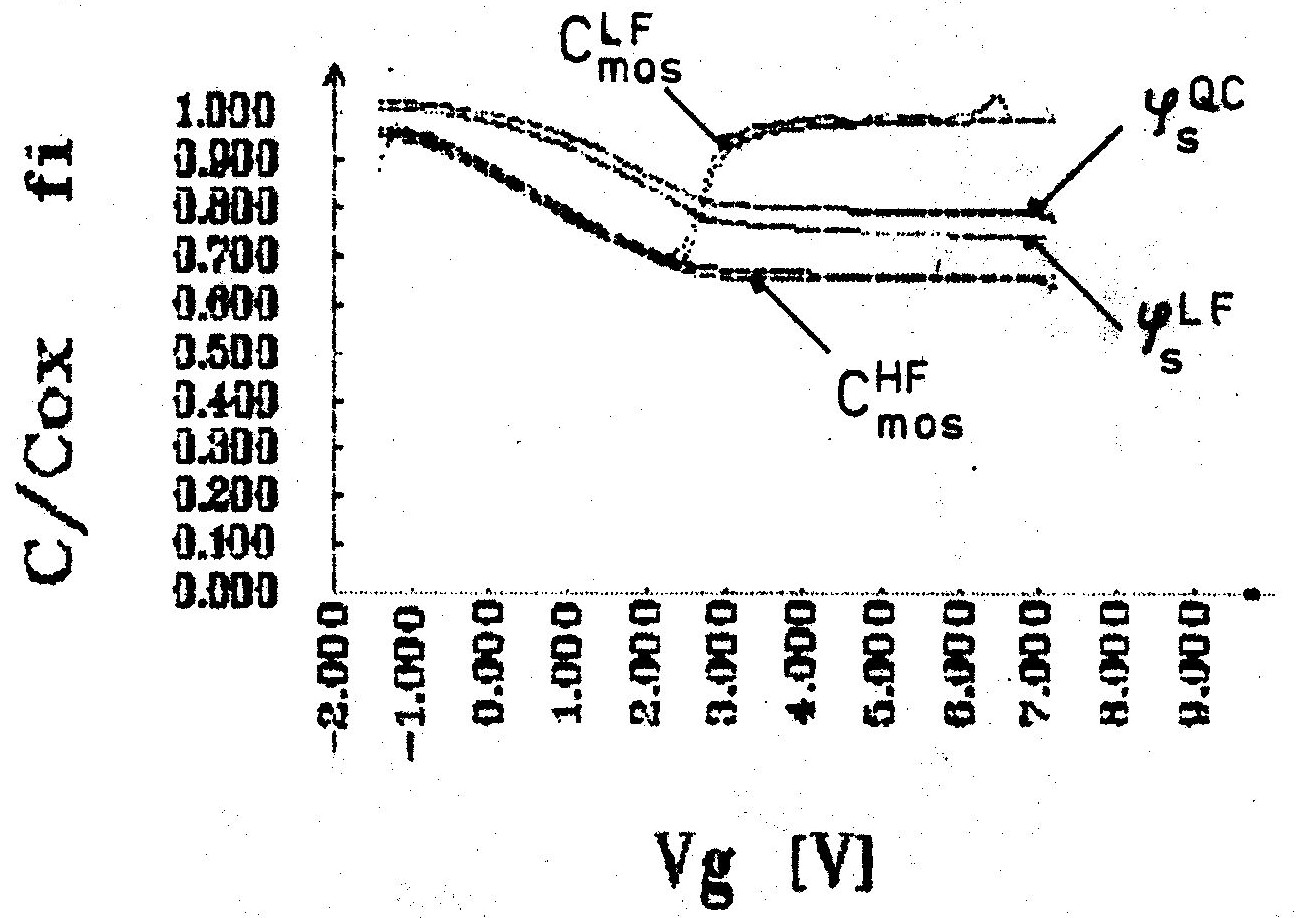
\includegraphics{Figures/fig-3-4.eps}
\captionsetup{justification=raggedright, singlelinecheck=false}
\caption[Normalized capacitance waveforms of MOS structure with substrate type
  P as a function of gate voltage for equilibrium high-frequency and
  quasi-static measurements]{Normalized capacitance waveforms of a MOS structure with
  P-type substrate as a function of gate voltage for equilibrium
  high-frequency and quasi-static measurements.  At the same time, those
  same characteristics obtained using the Q-C method. For completeness, the
  the dependence of the surface potential
  ${\varphi_s(V_g)}^{QC}$ obtained using the Q-C method and the dependence
  ${\varphi_s(V_g)}^{LF}$ calculated by integrating the low-frequency C-V
  dependence using the Berglund integral. Flows
  $\varphi_s(V_g)$ are shown using the normalization $1 -
  \frac{\varphi_s}{\varphi_{norm}}$, kde $\varphi_{norm}=3.33V$.}\label{fig:3.4}
\end{figure}
%OBR6.BIT

\begin{table}[h!]\centering
  \begin{tabular}{c c c c c c}
    \multicolumn{3}{l}{$C^{HF}_{mos}$} & \multicolumn{3}{l}{$C^{LF}_{mos}$} \\
    HF[\%] & QC[\%] & $\Delta_r$[\%] & LF[\%] & QC[\%] & $\Delta_r$[\%] \\
    \hline
    96.30 & 95.71 & +0.62 & 94.80 & 94.89 & -0.09 \\
    92.88 & 92.07 & +0.87 & 91.03 & 92.83 & -1.98 \\
    87.52 & 86.48 & +1.19 & 85.97 & 87.53 & -1.81 \\
    81.39 & 80.09 & +1.60 & 79.70 & 81.20 & -1.88 \\
    75.71 & 74.55 & +1.53 & 74.24 & 76.00 & -2.37 \\
    71.17 & 69.79 & +1.98 & 69.89 & 70.65 & -1.08 \\
    67.77 & 66.41 & +2.00 & 80.77 & 83.57 & -3.47 \\
    67.14 & 65.85 & +1.93 & 94.72 & 96.93 & -2.33 \\
    66.82 & 65.73 & +1.62 & 96.77 & 98.26 & -1.53 \\
    66.65 & 65.63 & +1.52 & 97.47 & 98.06 & -0.60 \\
    66.62 & 65.59 & +1.53 & 97.94 & 99.46 & -1.56 \\
    66.58 & 65.54 & +1.56 & 98.15 & 99.39 & -1.26 \\
  \end{tabular}
  \caption[Comparison of normalized frequency and low-frequency
    capacitance of the MOS structure (Figure~\ref{fig:3.4}) for HF, LF
    and Q-C methods]{Comparison of normalized high-frequency and
    low-frequency capacitance of the MOS structure
    (Figure~\ref{fig:3.4}) for HF, LF and Q-C methods. The difference
    of the curves is expressed by the relative error.}\label{tab:3.2}
\end{table}

\section{Constant-width OPN method and determination of the generation lifetime of minority charge carriers.}\label{sec:3.4}

The substrate quality of the MOS slit can be judged from the
generation time lifetime of the minority charge carriers, which we
will denote by $\tau_g$. The classical method of determining this
parameter is the Zerbst method~\cite{3.2}, which determines $\tau_g$
from the relaxation transition time of the MOS structure from the
non-equilibrium state to the equilibrium state. Currently the
semiconductor industry is working with high quality silicon wafers,
whose relaxation times are in the order of tens of minutes, which
precludes the effective use of the Zerbst method in controlling
semiconductor technology. Significant acceleration of the
determination process $\tau_g$ of high quality silicon substrates is
made possible by the constant width OPN~\cite{3.1}. Its principle is
as follows. The MOS structure is brought to a non-equilibrium state by
a voltage pulse at the gate of deep depletion. The generation of
minority charge carriers causes the formation of an inversion layer on
the semiconductor surface, shading the substrate and subsequent OPN
tapering, which is manifested by an increase in the capacitance of the
structure MOS\@. The effect of the generation of minority charge
carriers on the width of the OPN can be be compensated by increasing
the gate voltage and thus ensuring a constant width of the
OPN\@. Obviously, the rate of increase of the gate voltage will depend
on the rate of generation of minority charge carriers, which can be
expressed by the following relation~\cite{3.3}

\begin{equation}\label{eq:3.4}
  I_g = C_{ox} \frac{dV_g}{dt}
\end{equation}

where $I_g$ represents the generation current of minority charge carriers that
form the inverse layer.  The generational lifetime of the minority carriers
$\tau_g$ can then be expressed using the generation current $I_g$~\cite{3.3}

\begin{equation}\label{eq:3.5}
  \tau_g = \frac{qxn_i}{2I_g}
\end{equation}

In the above method, we assume that the charge increment in the
inverse layer is made up only of minority charge carriers that are
generated in the OPN\@. This neglects the diffusion of minority
carriers from the substrate and the surface of the semiconductor,
which may distort the measured results. Distortion results can occur
especially if the space in which the the measured sample is not
perfectly sealed, which causes ingress light in. The electron-hole
pairs generated by the photons trapped on the the surface of the
semiconductor, contribute to the generation current and the calculated
values of $\tau_g$ will be less than their actual value.  Impact of
the above phenomena can be eliminated if we determine $\tau_g$ from
the difference of the measured $V_g(t)$ dependence directions for
different widths OPN~\cite{3.3, 3.10, 3.11, 3.12}. The generation
current, formed by the minor charge carriers that are generated in the
OPN, can then be expressed by the relation

\begin{equation}\label{eq:3.6}
  I_g = C_{ox} \bigg[\frac{dV_g}{dt}\Big\rvert_{C_1} - \frac{dV_g}{dt}\Big\rvert_{C_2}\bigg]
\end{equation}

and the generation time $\tau_g$

\begin{equation}\label{eq:3.7}
  \tau_g = \frac{q\Delta x n_i}{2I_g}
\end{equation}

where $\Delta x$ is the distance by which the OPN is expanded when the
capacity changes from $C_1$ to $C_2$

\begin{equation}\label{eq:3.8}
  \Delta x = \epsilon \Big[\frac{1}{C_2} - \frac{1}{C_1}\Big]
\end{equation}

The calculated value of $\tau_g$ from the relation~\ref{eq:3.7} is
then the mean value of the generational lifetime of the minority
charge carriers in the region of the semiconductor defined by the
distance $\Delta x$.  Issues of nonequilibrium measurements has been
treated in our department in paper~\cite{1.6} and an analog
implementation of the above method has been has been treated in
Thesis~\cite{3.13}. Part of this dissertation is A numerical
implementation of the constant-width method OPN\@. In order to measure
capacitance was used to measure the HP4280a instrument, which also
contains a source of DC voltage source. The method was automated using
a bus IMS-2. The most important part of the control program is the
loop, in which maintains the constant capacitance of the MOS structure
in non-equilibrium state by varying the gate voltage.  If we know the
waveform concentration profile in the semiconductor, we can calculate
the necessary change gate voltage for a measured change in the
capacitance of the MOS structure from relation~\ref{eq:3.3}

\begin{equation}\label{eq:3.9}
  \frac{dV_g}{dC_{mos}} = \frac{q\epsilon N}{C^3_{mos}}
\end{equation}

If we measure time at the same time, we get the dependence
$V_g(t)$. Measurement procedure one dependence $V_g(t)$ is shown by
the following evolution diagram.

\begin{diagram}
  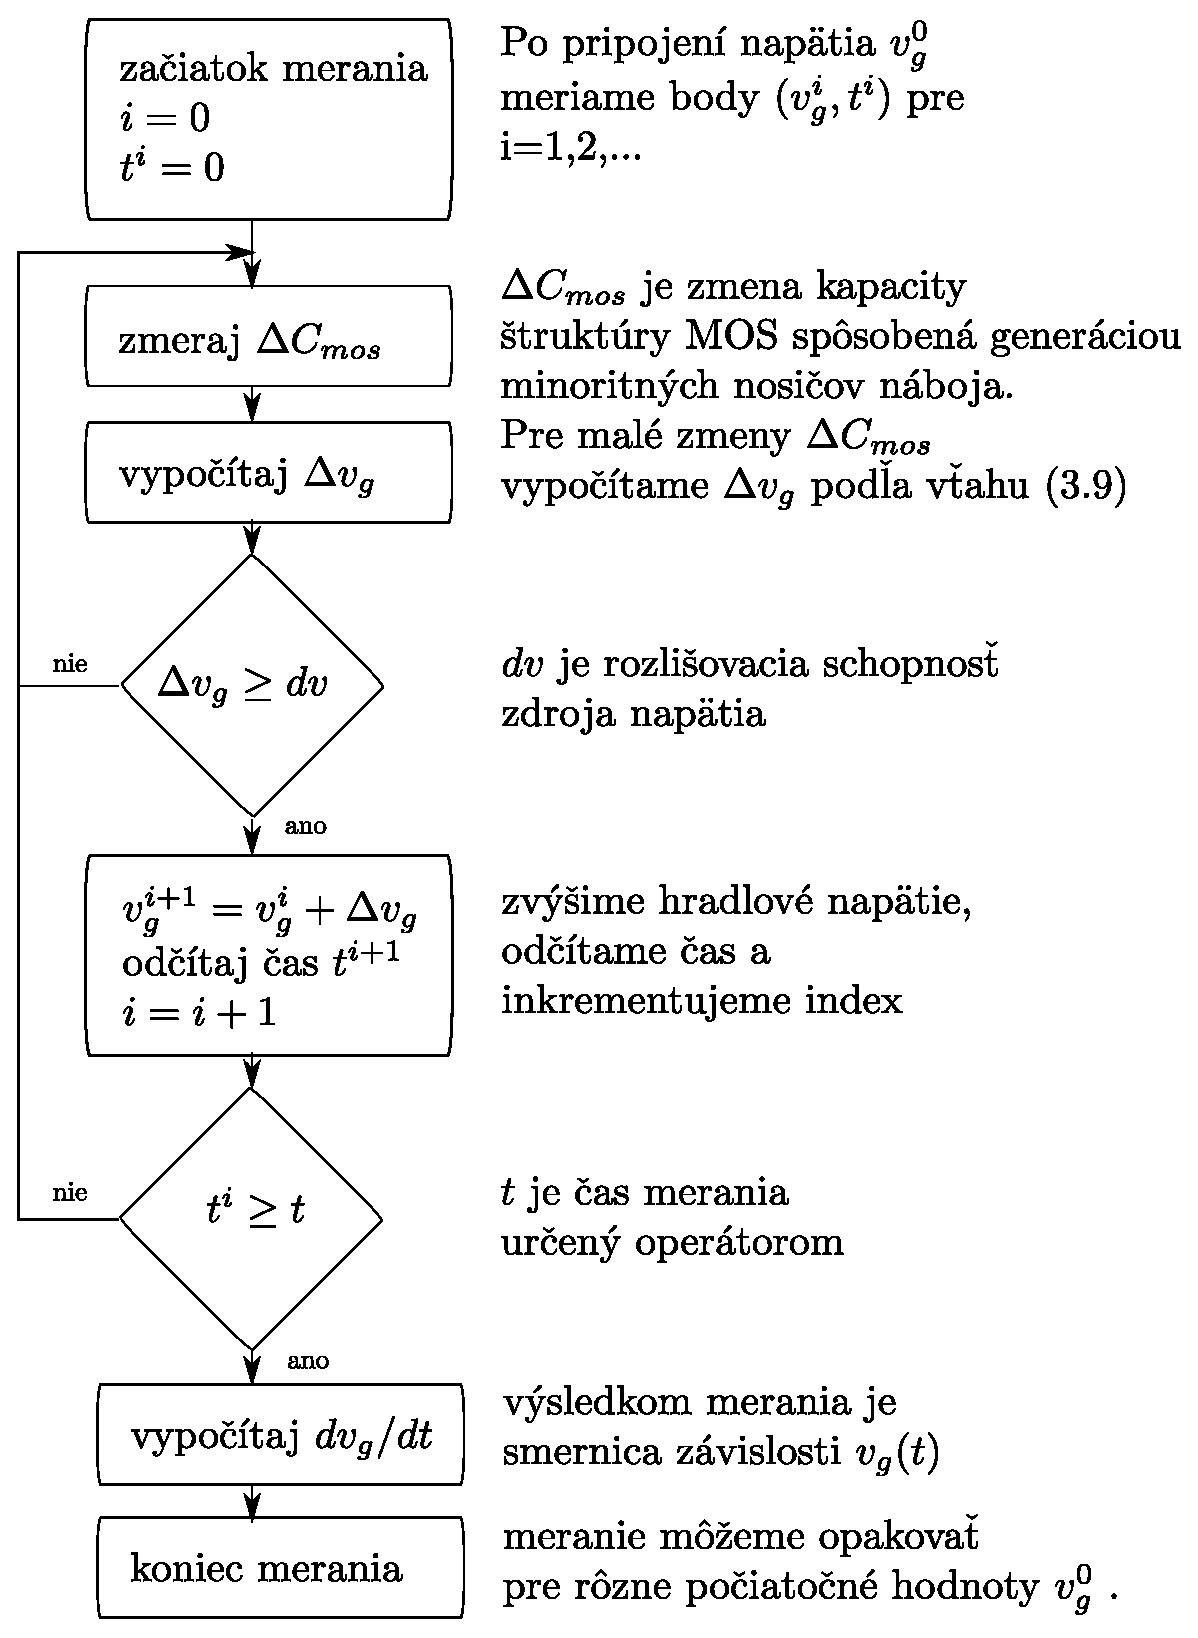
\includegraphics[scale=0.55,keepaspectratio]{Figures/diagram-2.EPS}\label{diagram:2}
\end{diagram}

\begin{figure}[h!]\centering
  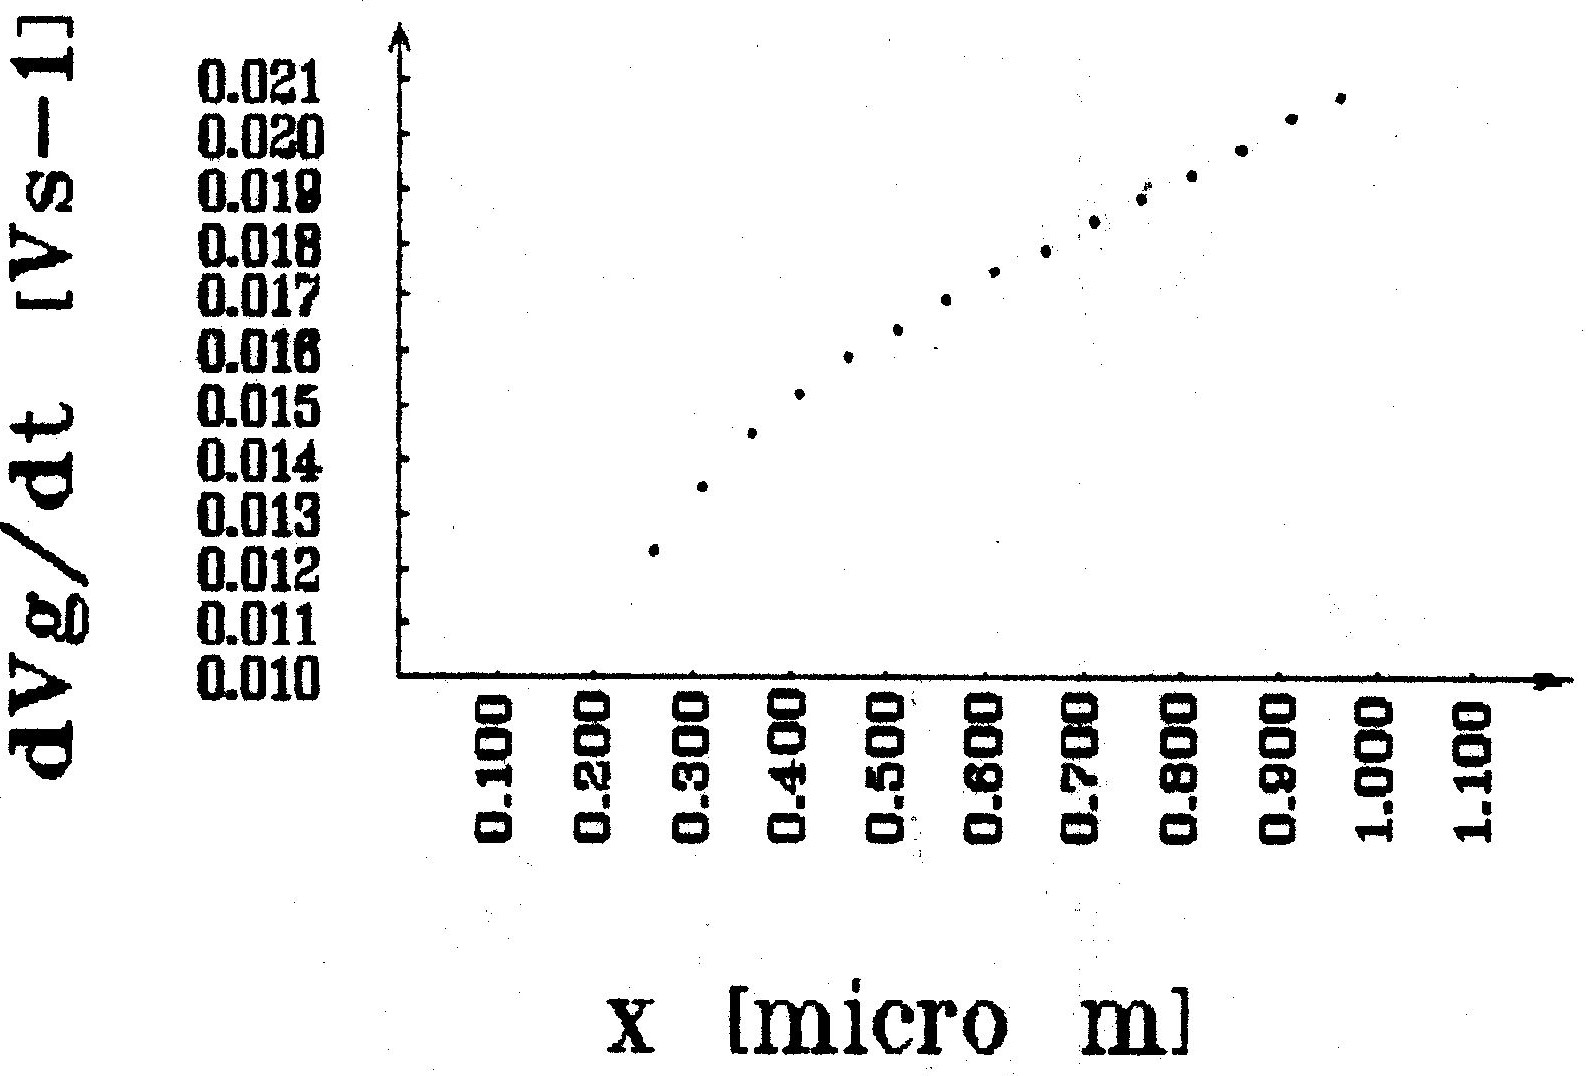
\includegraphics{Figures/fig-3-5.eps}
  \caption[Dependence of $\frac{dV_g}{dt}$ on OPN width obtained by
    constant OPN width method]{Dependence of $\frac{dV_g}{dt}$ on width
    OPN obtained using the constant width OPN method.}\label{fig:3.5}
\end{figure}
%OBR19.BIT

Figure~\ref{fig:3.5} shows the dependence of $\frac{dV_g}{dt}$ on
of the width of OPN\@. Assuming the OPN width is kept constant, the
potential ratios in the semiconductor and the generation of minority carriers is
constant, implying a linear dependence of $V_g(t)$.  Guidelines
${frac{dV_g}{dt}}$ can then be determined by linear regression of the measured
$V_g(t)$ dependence. It is not difficult to imagine that
relations~\ref{eq:3.6} to~\ref{eq:3.8} represent the discretization
of the continuous waveform $\tau_g(x)$. If the measured values
$\frac{dV_g}{dt}=f(x)$ are approximated by a continuous function, we can express
the depth profile $\tau_g(x)$ by the relation

\begin{equation}\label{eq:3.10}
  \tau_g(x) = \frac{qn_i}{2C_{ox}} {\Bigg[\frac{d\big[\frac{dV_g}{dt}\big]}{dx}\Bigg]}^{-1}
\end{equation}

Figure~\ref{fig:3.6} shows the waveform of $\tau_g(x)$, calculated
from the measured data shown in Figure~\ref{fig:3.5} and in
Figure~\ref{fig:3.7} is the depth concentration profile $N(x)$ of the investigated
structure.

\begin{figure}[h!]\centering
  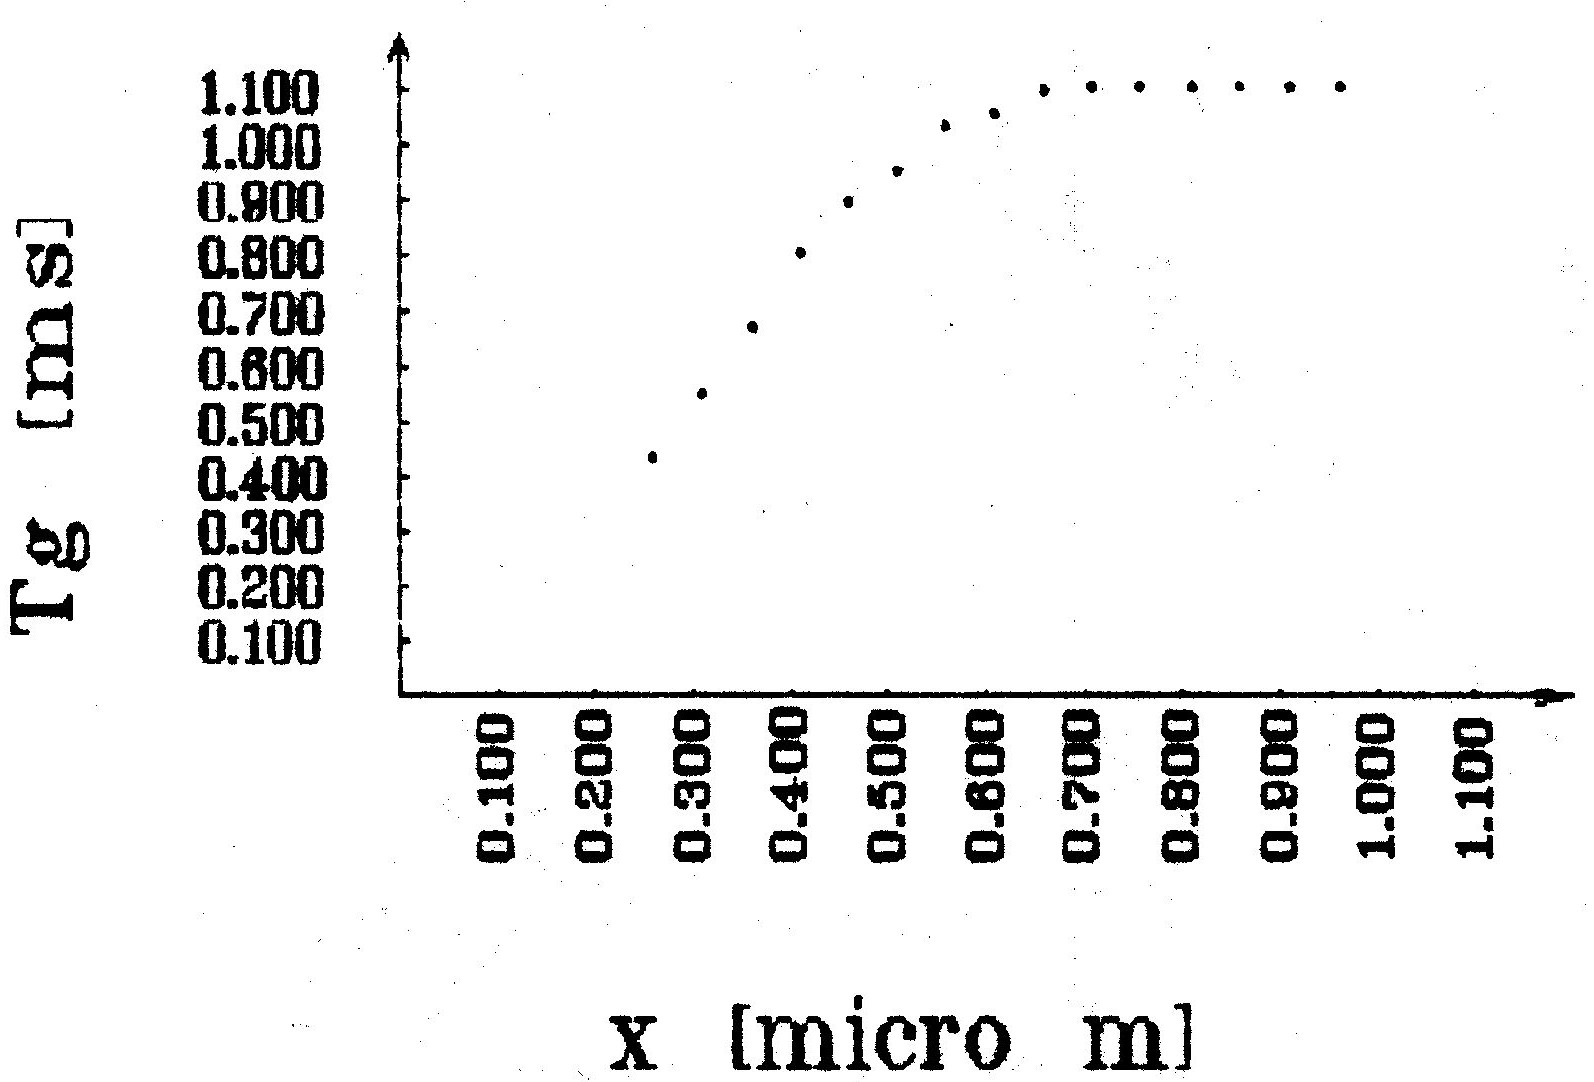
\includegraphics{Figures/fig-3-6.eps}
  \caption[Depth profile of the generation lifetime of minority carriers
    charge]{Depth profile of the generation time of minority carriers
    of the minority of the charge.}\label{fig:3.6}
\end{figure}
%OBR20.BIT

\begin{figure}[h!]\centering
  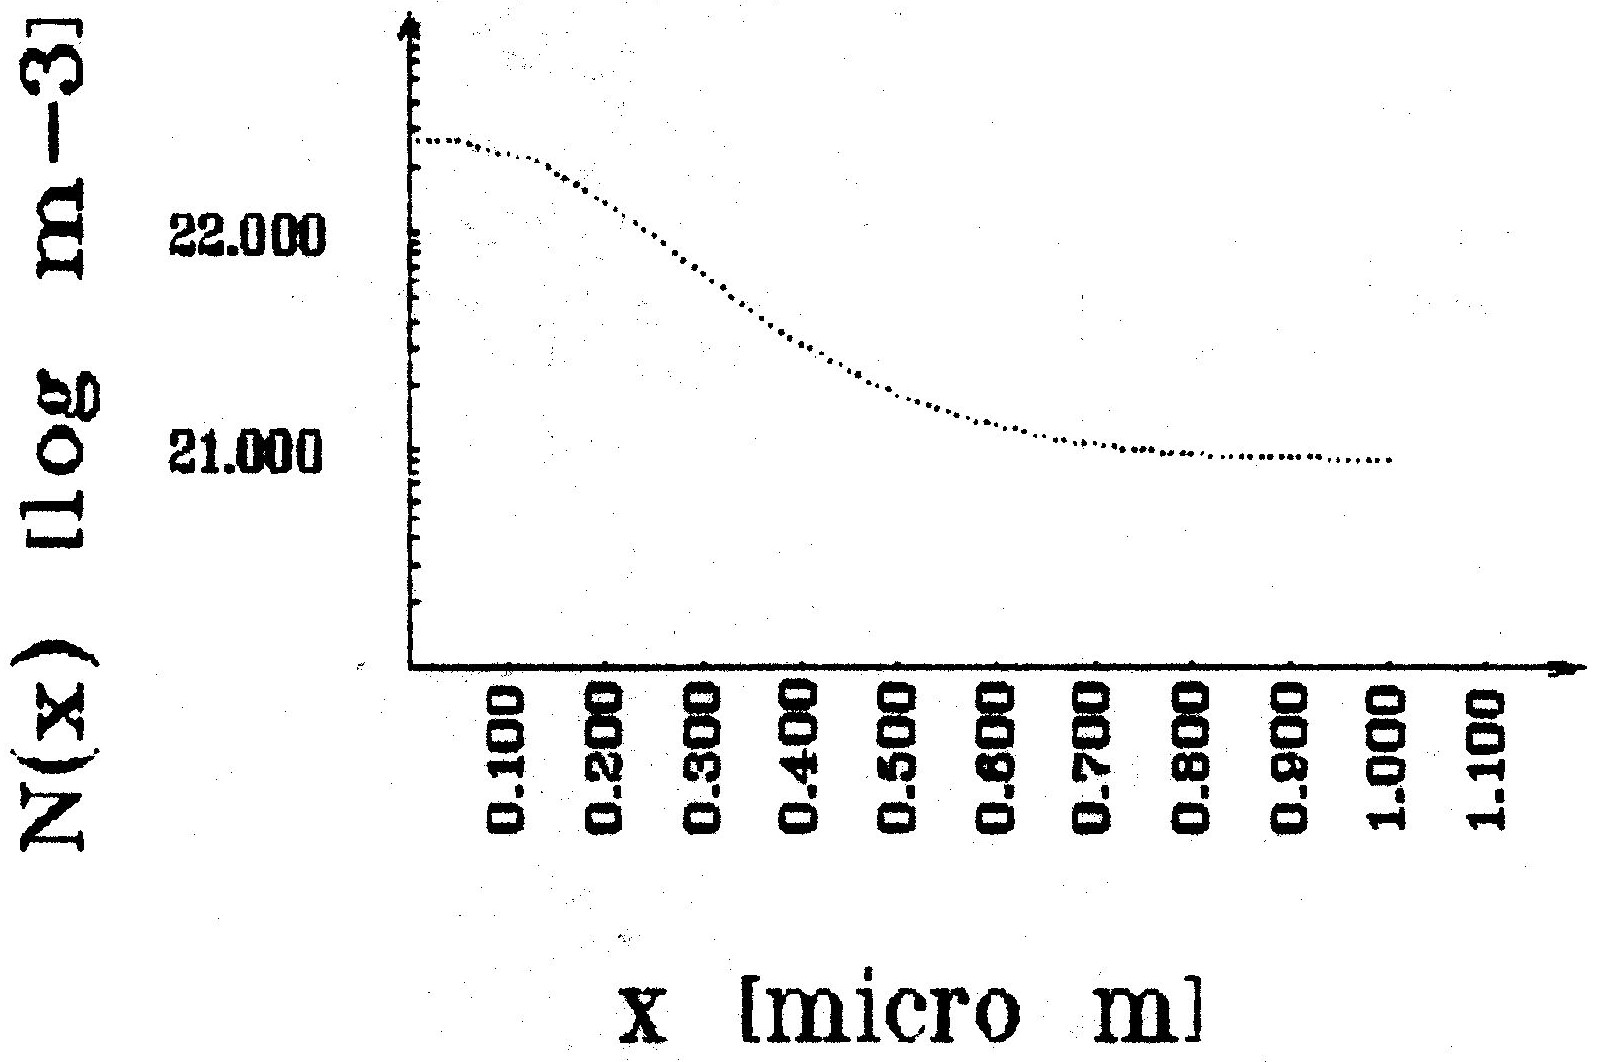
\includegraphics{Figures/fig-3-7.eps}
  \caption[Depth profile of concentration of interfering impurities
    $N(x)$]{Depth concentration profile of interfering impurities
    $N(x)$. The impurity concentration profile was created by implanting
    $P^{31}$ with a dose of $8.0$ $10^{15}m^{-2}$ at an energy of $120 keV$.
    The activation was carried out for 40 minutes at a temperature of $1050 \degree C$ in
    $N_2$ atmosphere.}\label{fig:3.7}
\end{figure}
%OBR21.BIT


\begin{thebibliography}{}

\bibitem[3.1]{3.1}
  Pierret R.F., Small D.W.: IEEE Trans.\ on elektron.dev. 22 (1975) s.1052.

\bibitem[3.2]{3.2}
  Zerbst M.. Angew. Phys. 22 (1966), p.30.

\bibitem[3.3]{3.3}
  Eades W.D., Shott J.D., Swanson R.M.: IEEE Trans.\ on elektron.\ dev. 30 (1983) s.1274.

\bibitem[3.4]{3.4}
  Nicollian E.H., Brews J.R.: Solid St.\ Electron.  27 (1984) s.953.

\bibitem[3.5]{3.5}
  Ziegler K., Klausmann E.: Appl. Phys. Lett. 26 (1975) p.400.

\bibitem[3.6]{3.6}
  Boulin D.M., Brews J.R., Nicollian E.H.: Solid St.\ Electron. 27 (1984) s.977.

\bibitem[3.7]{3.7}
  Brews J.R., Nicollian E.H.: Solid St.\ Electron. 27 (1984) s.963.

\bibitem[3.8]{3.8}
  Botka V.,Csabay O., Jamrich M.: 5th national conference Microelectronics 1989, House of Technology CSVTS Bratislava, 1989 p.59.

\bibitem[3.9]{3.9}
  Jamrich M.: Q-C method for the investigation of MIS\@ structures. Diploma thesis, Department of Microelectronics, EF SVŠT, Bratislava 1988.

\bibitem[3.10]{3.10}
  Beyer A., Markgraf W.: Wiss. Z. d. Techn. Hochsch. Karl-Marx-Stadt 28 (1986) p.479.

\bibitem[3.11]{3.11}
  Lal, Vasi: Solid St.\ Electron. 30 (1987) s.801.

\bibitem[3.12]{3.12}
  Hof, Morthers, Roenker: Solid St.\ Electron. 31 (1988) s.937.

\bibitem[3.13]{3.13}
  Pilka K.: Non-equilibrium capacitive method with constant width OPN, Department of Microelectronics, EF SVŠT, Bratislava 1989.

\end{thebibliography}
